\documentclass{standalone}
\usepackage{tikz}
\usetikzlibrary{patterns, positioning}
\usepackage[sfdefault]{ClearSans} %% option 'sfdefault' activates Clear Sans as the default text font
\usepackage[T1]{fontenc}

\begin{document}
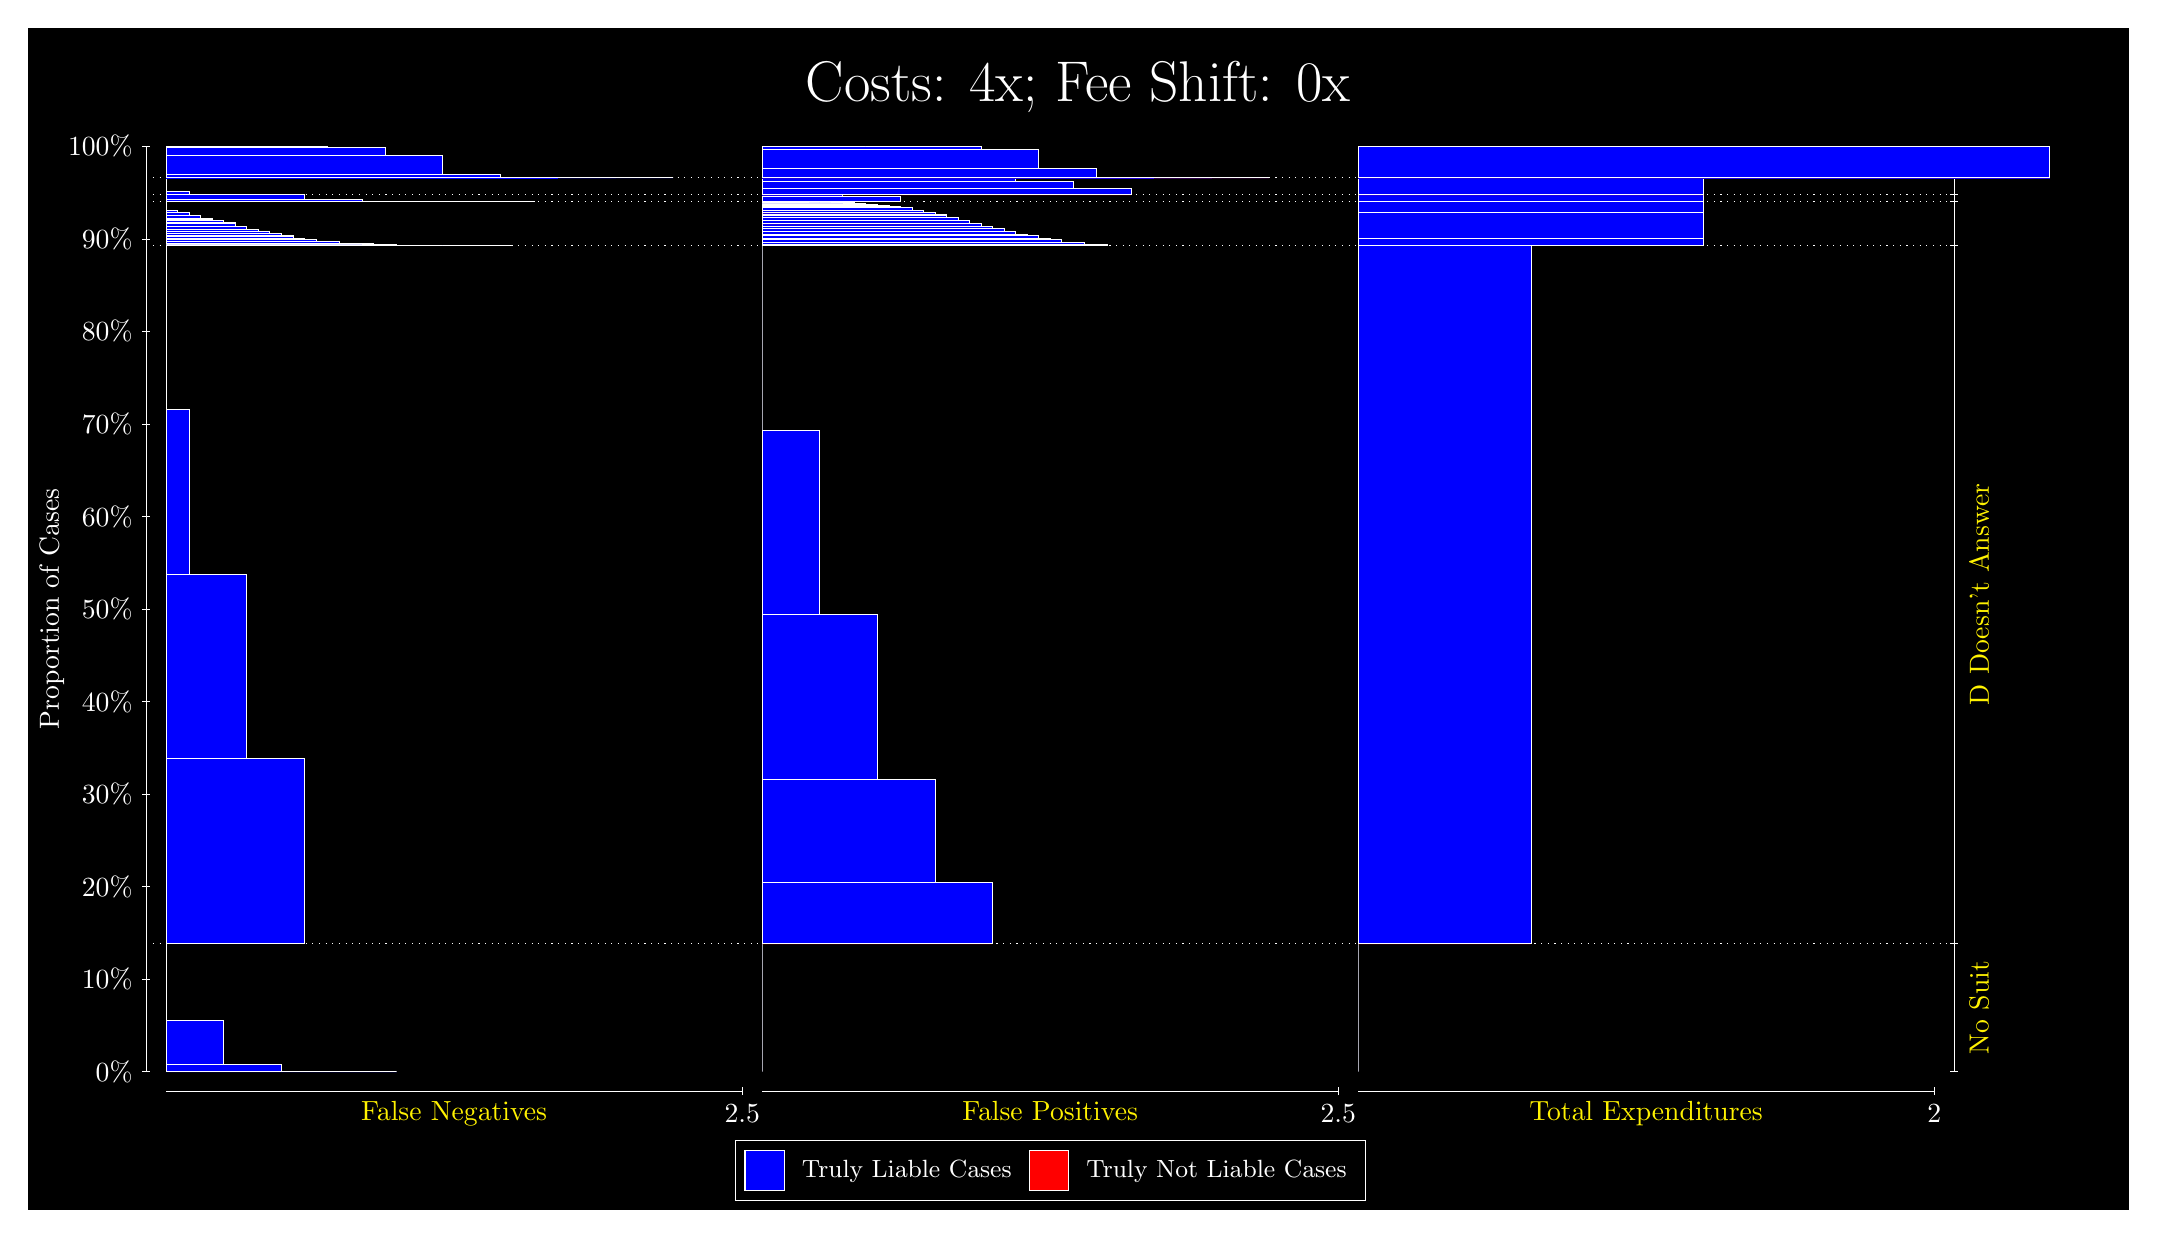
\begin{tikzpicture}
\draw[fill=black] (0,0) rectangle (26.667,15);
\draw[text=white] (0,13.5) rectangle (26.667,15) node[midway] {\huge Costs: 4x; Fee Shift: 0x};
\draw[white, very thin] (1.5,1.75) -- (1.5,13.5);
\node[rotate=90, text=white, anchor=center] at (0.3, 7.625) {Proportion of Cases};
\draw[white, very thin] (1.45,1.75) -- (1.55,1.75);
\node[text=white, anchor=east] at (1.45, 1.75) {0\%};
\draw[white, very thin] (1.45,2.925) -- (1.55,2.925);
\node[text=white, anchor=east] at (1.45, 2.925) {10\%};
\draw[white, very thin] (1.45,4.1) -- (1.55,4.1);
\node[text=white, anchor=east] at (1.45, 4.1) {20\%};
\draw[white, very thin] (1.45,5.275) -- (1.55,5.275);
\node[text=white, anchor=east] at (1.45, 5.275) {30\%};
\draw[white, very thin] (1.45,6.45) -- (1.55,6.45);
\node[text=white, anchor=east] at (1.45, 6.45) {40\%};
\draw[white, very thin] (1.45,7.625) -- (1.55,7.625);
\node[text=white, anchor=east] at (1.45, 7.625) {50\%};
\draw[white, very thin] (1.45,8.8) -- (1.55,8.8);
\node[text=white, anchor=east] at (1.45, 8.8) {60\%};
\draw[white, very thin] (1.45,9.975) -- (1.55,9.975);
\node[text=white, anchor=east] at (1.45, 9.975) {70\%};
\draw[white, very thin] (1.45,11.15) -- (1.55,11.15);
\node[text=white, anchor=east] at (1.45, 11.15) {80\%};
\draw[white, very thin] (1.45,12.325) -- (1.55,12.325);
\node[text=white, anchor=east] at (1.45, 12.325) {90\%};
\draw[white, very thin] (1.45,13.5) -- (1.55,13.5);
\node[text=white, anchor=east] at (1.45, 13.5) {100\%};

\draw[white, very thin] (24.457,1.75) -- (24.457,13.5);
\draw[white, very thin] (24.407,1.75) -- (24.507,1.75);
\node[anchor=west] at (24.407, 1.75) {};
\draw[white, very thin] (24.407,3.3738) -- (24.507,3.3738);
\node[anchor=west] at (24.407, 3.3738) {};
\draw[white, very thin] (24.407,12.245) -- (24.507,12.245);
\node[anchor=west] at (24.407, 12.245) {};
\draw[white, very thin] (24.407,12.803) -- (24.507,12.803);
\node[anchor=west] at (24.407, 12.803) {};
\draw[white, very thin] (24.407,12.887) -- (24.507,12.887);
\node[anchor=west] at (24.407, 12.887) {};
\draw[white, very thin] (24.407,13.102) -- (24.507,13.102);
\node[anchor=west] at (24.407, 13.102) {};
\draw[white, very thin] (24.407,13.5) -- (24.507,13.5);
\node[anchor=west] at (24.407, 13.5) {};

\draw[white, very thin, fill=blue] (1.75,1.75) rectangle (4.6775,1.75);
\draw[white, very thin, fill=blue] (1.75,1.75) rectangle (3.9457,1.7508);
\draw[white, very thin, fill=blue] (1.75,1.7508) rectangle (3.2138,1.8429);
\draw[white, very thin, fill=blue] (1.75,1.8429) rectangle (2.4819,2.4044);
\draw[white, very thin, fill=red] (1.75,2.4044) rectangle (1.75,2.4044);
\draw[white, very thin, fill=blue] (1.75,2.4044) rectangle (1.75,3.3738);
\draw[white, very thin, fill=blue] (1.75,3.3738) rectangle (3.5065,5.7236);
\draw[white, very thin, fill=blue] (1.75,5.7236) rectangle (2.7746,8.0594);
\draw[white, very thin, fill=blue] (1.75,8.0594) rectangle (2.0428,10.163);
\draw[white, very thin, fill=red] (1.75,10.163) rectangle (1.75,10.163);
\draw[white, very thin, fill=blue] (1.75,10.163) rectangle (1.75,12.245);
\draw[white, very thin, fill=blue] (1.75,12.245) rectangle (6.1413,12.245);
\draw[white, very thin, fill=blue] (1.75,12.245) rectangle (5.8486,12.245);
\draw[white, very thin, fill=blue] (1.75,12.245) rectangle (5.5558,12.245);
\draw[white, very thin, fill=blue] (1.75,12.245) rectangle (5.4094,12.246);
\draw[white, very thin, fill=blue] (1.75,12.246) rectangle (5.2631,12.246);
\draw[white, very thin, fill=blue] (1.75,12.246) rectangle (5.1167,12.246);
\draw[white, very thin, fill=blue] (1.75,12.246) rectangle (4.9703,12.246);
\draw[white, very thin, fill=blue] (1.75,12.246) rectangle (4.8239,12.246);
\draw[white, very thin, fill=blue] (1.75,12.246) rectangle (4.6775,12.255);
\draw[white, very thin, fill=blue] (1.75,12.255) rectangle (4.5312,12.256);
\draw[white, very thin, fill=blue] (1.75,12.256) rectangle (4.3848,12.256);
\draw[white, very thin, fill=blue] (1.75,12.256) rectangle (4.3848,12.263);
\draw[white, very thin, fill=blue] (1.75,12.263) rectangle (4.2384,12.263);
\draw[white, very thin, fill=blue] (1.75,12.263) rectangle (4.092,12.272);
\draw[white, very thin, fill=blue] (1.75,12.272) rectangle (4.092,12.272);
\draw[white, very thin, fill=blue] (1.75,12.272) rectangle (3.9457,12.291);
\draw[white, very thin, fill=blue] (1.75,12.291) rectangle (3.7993,12.299);
\draw[white, very thin, fill=blue] (1.75,12.299) rectangle (3.6529,12.3);
\draw[white, very thin, fill=blue] (1.75,12.3) rectangle (3.6529,12.315);
\draw[white, very thin, fill=blue] (1.75,12.315) rectangle (3.5065,12.326);
\draw[white, very thin, fill=blue] (1.75,12.326) rectangle (3.3602,12.363);
\draw[white, very thin, fill=blue] (1.75,12.363) rectangle (3.3602,12.364);
\draw[white, very thin, fill=blue] (1.75,12.364) rectangle (3.2138,12.391);
\draw[white, very thin, fill=blue] (1.75,12.391) rectangle (3.0674,12.4);
\draw[white, very thin, fill=blue] (1.75,12.4) rectangle (3.0674,12.416);
\draw[white, very thin, fill=blue] (1.75,12.416) rectangle (2.921,12.427);
\draw[white, very thin, fill=blue] (1.75,12.427) rectangle (2.921,12.447);
\draw[white, very thin, fill=blue] (1.75,12.447) rectangle (2.7746,12.484);
\draw[white, very thin, fill=blue] (1.75,12.484) rectangle (2.6283,12.523);
\draw[white, very thin, fill=blue] (1.75,12.523) rectangle (2.6283,12.532);
\draw[white, very thin, fill=blue] (1.75,12.532) rectangle (2.4819,12.56);
\draw[white, very thin, fill=blue] (1.75,12.56) rectangle (2.3355,12.569);
\draw[white, very thin, fill=blue] (1.75,12.569) rectangle (2.3355,12.587);
\draw[white, very thin, fill=blue] (1.75,12.587) rectangle (2.1891,12.622);
\draw[white, very thin, fill=blue] (1.75,12.622) rectangle (2.0428,12.662);
\draw[white, very thin, fill=blue] (1.75,12.662) rectangle (1.8964,12.684);
\draw[white, very thin, fill=red] (1.75,12.684) rectangle (1.75,12.684);
\draw[white, very thin, fill=blue] (1.75,12.684) rectangle (1.75,12.803);
\draw[white, very thin, fill=blue] (1.75,12.803) rectangle (6.4341,12.803);
\draw[white, very thin, fill=blue] (1.75,12.803) rectangle (5.7022,12.803);
\draw[white, very thin, fill=blue] (1.75,12.803) rectangle (4.9703,12.805);
\draw[white, very thin, fill=blue] (1.75,12.805) rectangle (4.2384,12.828);
\draw[white, very thin, fill=blue] (1.75,12.828) rectangle (3.5065,12.887);
\draw[white, very thin, fill=red] (1.75,12.887) rectangle (1.75,12.887);
\draw[white, very thin, fill=blue] (1.75,12.887) rectangle (3.5065,12.887);
\draw[white, very thin, fill=blue] (1.75,12.887) rectangle (2.7746,12.893);
\draw[white, very thin, fill=blue] (1.75,12.893) rectangle (2.0428,12.934);
\draw[white, very thin, fill=red] (1.75,12.934) rectangle (1.75,12.934);
\draw[white, very thin, fill=blue] (1.75,12.934) rectangle (1.75,13.102);
\draw[white, very thin, fill=blue] (1.75,13.102) rectangle (8.1906,13.102);
\draw[white, very thin, fill=blue] (1.75,13.102) rectangle (7.4587,13.102);
\draw[white, very thin, fill=blue] (1.75,13.102) rectangle (6.7268,13.103);
\draw[white, very thin, fill=blue] (1.75,13.103) rectangle (5.9949,13.145);
\draw[white, very thin, fill=blue] (1.75,13.145) rectangle (5.2631,13.38);
\draw[white, very thin, fill=blue] (1.75,13.38) rectangle (4.5312,13.489);
\draw[white, very thin, fill=blue] (1.75,13.489) rectangle (3.7993,13.5);
\draw[white, very thin, fill=blue] (1.75,13.5) rectangle (3.0674,13.5);
\draw[white, very thin, fill=blue] (1.75,13.5) rectangle (2.3355,13.5);
\draw[white, very thin, fill=red] (1.75,13.5) rectangle (1.75,13.5);
\draw[white, very thin, fill=red] (9.3189,1.75) rectangle (9.3189,1.75);
\draw[white, very thin, fill=blue] (9.3189,1.75) rectangle (9.3189,3.3738);
\draw[white, very thin, fill=red] (9.3189,3.3738) rectangle (12.246,3.3738);
\draw[white, very thin, fill=blue] (9.3189,3.3738) rectangle (12.246,4.1544);
\draw[white, very thin, fill=blue] (9.3189,4.1544) rectangle (11.515,5.4557);
\draw[white, very thin, fill=blue] (9.3189,5.4557) rectangle (10.783,7.5597);
\draw[white, very thin, fill=blue] (9.3189,7.5597) rectangle (10.051,9.8955);
\draw[white, very thin, fill=blue] (9.3189,9.8955) rectangle (9.3189,12.245);
\draw[white, very thin, fill=red] (9.3189,12.245) rectangle (13.71,12.245);
\draw[white, very thin, fill=blue] (9.3189,12.245) rectangle (13.71,12.26);
\draw[white, very thin, fill=red] (9.3189,12.26) rectangle (13.417,12.26);
\draw[white, very thin, fill=blue] (9.3189,12.26) rectangle (13.417,12.282);
\draw[white, very thin, fill=red] (9.3189,12.282) rectangle (13.125,12.282);
\draw[white, very thin, fill=blue] (9.3189,12.282) rectangle (13.125,12.322);
\draw[white, very thin, fill=blue] (9.3189,12.322) rectangle (12.978,12.333);
\draw[white, very thin, fill=red] (9.3189,12.333) rectangle (12.832,12.333);
\draw[white, very thin, fill=blue] (9.3189,12.333) rectangle (12.832,12.364);
\draw[white, very thin, fill=blue] (9.3189,12.364) rectangle (12.686,12.386);
\draw[white, very thin, fill=red] (9.3189,12.386) rectangle (12.539,12.386);
\draw[white, very thin, fill=blue] (9.3189,12.386) rectangle (12.539,12.427);
\draw[white, very thin, fill=blue] (9.3189,12.427) rectangle (12.393,12.462);
\draw[white, very thin, fill=red] (9.3189,12.462) rectangle (12.246,12.462);
\draw[white, very thin, fill=blue] (9.3189,12.462) rectangle (12.246,12.488);
\draw[white, very thin, fill=blue] (9.3189,12.488) rectangle (12.1,12.517);
\draw[white, very thin, fill=red] (9.3189,12.517) rectangle (11.954,12.517);
\draw[white, very thin, fill=blue] (9.3189,12.517) rectangle (11.954,12.565);
\draw[white, very thin, fill=blue] (9.3189,12.565) rectangle (11.807,12.602);
\draw[white, very thin, fill=red] (9.3189,12.602) rectangle (11.661,12.602);
\draw[white, very thin, fill=blue] (9.3189,12.602) rectangle (11.661,12.621);
\draw[white, very thin, fill=blue] (9.3189,12.621) rectangle (11.661,12.633);
\draw[white, very thin, fill=blue] (9.3189,12.633) rectangle (11.515,12.658);
\draw[white, very thin, fill=red] (9.3189,12.658) rectangle (11.368,12.658);
\draw[white, very thin, fill=blue] (9.3189,12.658) rectangle (11.368,12.685);
\draw[white, very thin, fill=blue] (9.3189,12.685) rectangle (11.222,12.723);
\draw[white, very thin, fill=blue] (9.3189,12.723) rectangle (11.075,12.733);
\draw[white, very thin, fill=blue] (9.3189,12.733) rectangle (10.929,12.749);
\draw[white, very thin, fill=blue] (9.3189,12.749) rectangle (10.929,12.75);
\draw[white, very thin, fill=blue] (9.3189,12.75) rectangle (10.783,12.758);
\draw[white, very thin, fill=blue] (9.3189,12.758) rectangle (10.636,12.776);
\draw[white, very thin, fill=blue] (9.3189,12.776) rectangle (10.49,12.786);
\draw[white, very thin, fill=blue] (9.3189,12.786) rectangle (10.344,12.786);
\draw[white, very thin, fill=blue] (9.3189,12.786) rectangle (10.197,12.793);
\draw[white, very thin, fill=blue] (9.3189,12.793) rectangle (10.197,12.793);
\draw[white, very thin, fill=blue] (9.3189,12.793) rectangle (10.051,12.793);
\draw[white, very thin, fill=blue] (9.3189,12.793) rectangle (9.9044,12.803);
\draw[white, very thin, fill=blue] (9.3189,12.803) rectangle (9.758,12.803);
\draw[white, very thin, fill=blue] (9.3189,12.803) rectangle (9.6116,12.803);
\draw[white, very thin, fill=blue] (9.3189,12.803) rectangle (9.4652,12.803);
\draw[white, very thin, fill=blue] (9.3189,12.803) rectangle (9.3189,12.803);
\draw[white, very thin, fill=red] (9.3189,12.803) rectangle (11.075,12.803);
\draw[white, very thin, fill=blue] (9.3189,12.803) rectangle (11.075,12.862);
\draw[white, very thin, fill=blue] (9.3189,12.862) rectangle (10.344,12.886);
\draw[white, very thin, fill=blue] (9.3189,12.886) rectangle (9.6116,12.887);
\draw[white, very thin, fill=blue] (9.3189,12.887) rectangle (9.3189,12.887);
\draw[white, very thin, fill=red] (9.3189,12.887) rectangle (14.003,12.887);
\draw[white, very thin, fill=blue] (9.3189,12.887) rectangle (14.003,12.961);
\draw[white, very thin, fill=blue] (9.3189,12.961) rectangle (13.271,13.054);
\draw[white, very thin, fill=blue] (9.3189,13.054) rectangle (12.539,13.096);
\draw[white, very thin, fill=blue] (9.3189,13.096) rectangle (11.807,13.102);
\draw[white, very thin, fill=blue] (9.3189,13.102) rectangle (11.075,13.102);
\draw[white, very thin, fill=red] (9.3189,13.102) rectangle (15.759,13.102);
\draw[white, very thin, fill=blue] (9.3189,13.102) rectangle (15.759,13.102);
\draw[white, very thin, fill=blue] (9.3189,13.102) rectangle (15.028,13.102);
\draw[white, very thin, fill=red] (9.3189,13.102) rectangle (15.028,13.102);
\draw[white, very thin, fill=blue] (9.3189,13.102) rectangle (15.028,13.102);
\draw[white, very thin, fill=blue] (9.3189,13.102) rectangle (14.296,13.103);
\draw[white, very thin, fill=red] (9.3189,13.103) rectangle (14.296,13.103);
\draw[white, very thin, fill=blue] (9.3189,13.103) rectangle (14.296,13.113);
\draw[white, very thin, fill=blue] (9.3189,13.113) rectangle (13.564,13.113);
\draw[white, very thin, fill=red] (9.3189,13.113) rectangle (13.564,13.113);
\draw[white, very thin, fill=blue] (9.3189,13.113) rectangle (13.564,13.222);
\draw[white, very thin, fill=blue] (9.3189,13.222) rectangle (12.832,13.222);
\draw[white, very thin, fill=red] (9.3189,13.222) rectangle (12.832,13.222);
\draw[white, very thin, fill=blue] (9.3189,13.222) rectangle (12.832,13.457);
\draw[white, very thin, fill=blue] (9.3189,13.457) rectangle (12.1,13.499);
\draw[white, very thin, fill=blue] (9.3189,13.499) rectangle (11.368,13.5);
\draw[white, very thin, fill=blue] (9.3189,13.5) rectangle (10.636,13.5);
\draw[white, very thin, fill=blue] (9.3189,13.5) rectangle (9.9044,13.5);
\draw[white, very thin, fill=red] (16.888,1.75) rectangle (16.888,1.75);
\draw[white, very thin, fill=blue] (16.888,1.75) rectangle (16.888,3.3738);
\draw[white, very thin, fill=red] (16.888,3.3738) rectangle (19.083,3.3738);
\draw[white, very thin, fill=blue] (16.888,3.3738) rectangle (19.083,12.245);
\draw[white, very thin, fill=red] (16.888,12.245) rectangle (21.279,12.245);
\draw[white, very thin, fill=blue] (16.888,12.245) rectangle (21.279,12.333);
\draw[white, very thin, fill=red] (16.888,12.333) rectangle (21.279,12.333);
\draw[white, very thin, fill=blue] (16.888,12.333) rectangle (21.279,12.661);
\draw[white, very thin, fill=red] (16.888,12.661) rectangle (21.279,12.661);
\draw[white, very thin, fill=blue] (16.888,12.661) rectangle (21.279,12.803);
\draw[white, very thin, fill=red] (16.888,12.803) rectangle (21.279,12.803);
\draw[white, very thin, fill=blue] (16.888,12.803) rectangle (21.279,12.887);
\draw[white, very thin, fill=red] (16.888,12.887) rectangle (21.279,12.887);
\draw[white, very thin, fill=blue] (16.888,12.887) rectangle (21.279,13.102);
\draw[white, very thin, fill=red] (16.888,13.102) rectangle (25.67,13.102);
\draw[white, very thin, fill=blue] (16.888,13.102) rectangle (25.67,13.104);
\draw[white, very thin, fill=red] (16.888,13.104) rectangle (25.67,13.104);
\draw[white, very thin, fill=blue] (16.888,13.104) rectangle (25.67,13.5);
\draw[white, dotted] (1.5,3.3738) -- (24.457,3.3738);
\draw[white, dotted] (1.5,12.245) -- (24.457,12.245);
\draw[white, dotted] (1.5,12.803) -- (24.457,12.803);
\draw[white, dotted] (1.5,12.887) -- (24.457,12.887);
\draw[white, dotted] (1.5,13.102) -- (24.457,13.102);
\draw[white, very thin] (1.75,1.5) -- (9.0689,1.5);
\node[text=yellow, anchor=north] at (5.4094, 1.5) {False Negatives};
\draw[white, very thin] (9.0689,1.45) -- (9.0689,1.55);
\node[text=white, anchor=north] at (9.0689, 1.45) {2.5};

\draw[white, very thin] (9.3189,1.5) -- (16.638,1.5);
\node[text=yellow, anchor=north] at (12.978, 1.5) {False Positives};
\draw[white, very thin] (16.638,1.45) -- (16.638,1.55);
\node[text=white, anchor=north] at (16.638, 1.45) {2.5};

\draw[white, very thin] (16.888,1.5) -- (24.207,1.5);
\node[text=yellow, anchor=north] at (20.547, 1.5) {Total Expenditures};
\draw[white, very thin] (24.207,1.45) -- (24.207,1.55);
\node[text=white, anchor=north] at (24.207, 1.45) {2};

\node[text=yellow, centered, rotate=90] at (24.777, 2.5619) {No Suit};
\node[text=yellow, centered, rotate=90] at (24.777, 7.8095) {D Doesn't Answer};





\draw (12.978300999999998,1.5) node[draw=none] (baseCoordinate) {};
\begin{scope}[align=center]
        \matrix[scale=0.5, draw=white, below=0.5cm of baseCoordinate, nodes={draw}, column sep=0.1cm]{
            \node[rectangle, draw, minimum width=0.5cm, minimum height=0.5cm, fill=blue] {}; &
            \node[draw=none, font=\small, text=white] (B) {Truly Liable Cases}; &
            \node[rectangle, draw, minimum width=0.5cm, minimum height=0.5cm, fill=red] {}; &
            \node[draw=none, font=\small, text=white] (B) {Truly Not Liable Cases}; \\
            };
\end{scope}

\end{tikzpicture}
\end{document}